\chapter{Elementi di metrologia e fondamenti della misurazione}

\begin{figure}[h]
    \centering
    \includegraphics[scale = 0.45]{Misurare è conoscere.PNG}
\end{figure}  
    
\newpage 

\section{Misura e misurazione} 
\footnote{Slide della prof | SDME 1.2 Metrologia - Introduzione | pag 2-4 }

Essendo il corso chiamato "Strumentazione Digitale e Misure Elettroniche", 
è fondamentale capire cosa significa misura. \newline 

Per misura, o meglio definirla come procedimento di misura, è quel procedimento 
che porta ad assegnare un valore ad una grandezza fisica detta misurando. \newline 

Alcune osservazioni riguardo al procedimento di misura: 

\begin{itemize}
    \item Il valore assegnato al misurando è parte essenziale ma non unico del risultato di misura 
    \item La maggior parte dei procedimento di misura viene effettuata per confronto 
    \item Esistono grandezze estensive e intensive
\end{itemize}


Il risultato della misurazione è l'informazione espressa da un valore numerico, una incertezza di misura 
e dalla corrispondente unità di misura. \newline 

Si può graficare il procedimento di misura come: 

\begin{figure}[h]
    \centering
    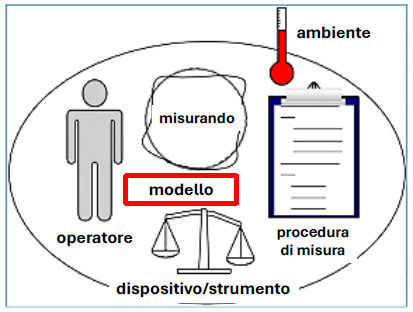
\includegraphics[scale = 0.6]{Procedimento di misura.PNG}
\end{figure}

Il metodo di misura per confronto con un riferimento o campione (unità) di misura indica 
che la quantità misurata Q si può esprimere: 

{
    \Large 
    \begin{equation}
        Q = VAL \cdot [U]
    \end{equation}
    
}

cioè un prodotto tra un valore numerico VAL e il campione o l'unità di misura [U]. \newline 

L'unità di misura è convenzionalmente una grandezza di valore unitario. \newline 

\newpage 

\section{La misurazione ideale e reale}
\footnote{Slide della prof | SDME 1.2 Metrologia - Introduzione | pag 5}


Secondo la norma UNI 4546, la misura è una informazione costituita da un valore, una incertezza ed una unità di misura, 
assegnata per rappresentare un parametro in un determinato stato del sistema. \newline 

La misurazione è un processo che mette in corrispondenza due insiemi: 
quello "reale" degli eventi fisici e quello "astratto" dei numeri. \newline 

Lo scopo della misurazione è fornire una descrizione rigorosa, quindi non soggettiva. \newline 

Utilizzando i grafici, la relazione tra il processo reale di misurazione e il mondo astratto è il seguente: 

\begin{figure}[h]
    \centering
    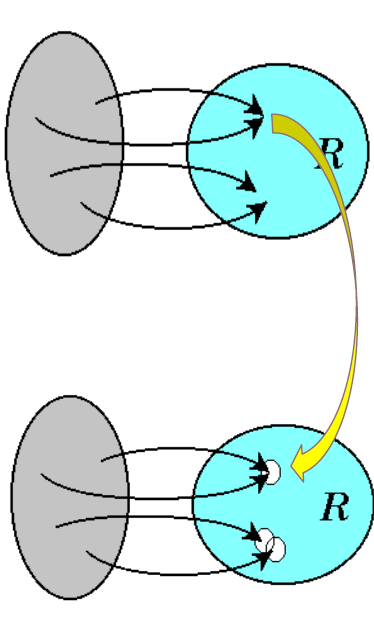
\includegraphics[scale = 0.5]{Misurazione ideale e reale.PNG}
\end{figure}

Come possiamo osservare, il processo reale di misurazione mette in corrispondenza ogni elemento 
dell'insieme degli eventi fisici con un sottoinsieme dell'insieme dei numeri. \newline 

Ciascun intervallo così determinato risulta centrato sul numero che rappresenta il "valore" del misurando. \newline 

La ampiezza dell'intervallo viene chiamata "incertezza" della misura. \newline 

\newpage 

\section{Definizione di grandezza}
\footnote{Slide della prof | SDME 1.2 Metrologia - Introduzione | pag 9}

Per grandezza si intende una quantità, proprietà, condizione usata per descrivere fenomeni e valutabile in termini di unità di misura. \newline 

Grandezza e misurando non sono la stessa cosa. \newline 

Per misurando si intende l'oggetto di una misurazione. \newline 

Le grandezze misurabili sono classificabili in 5 tipi: 

\begin{itemize}
    \item Numerale: numerazione di oggetti o singoli eventi singoli 
    \item Razionale: valori espressi da numeri razionali, cioè il rapporto tra grandezza misurata e u.d.m (unità di misura) 
    \item Strumentale: valori espressi come corrispondenza biunivoca con punti di scale convenzionali interpolabili 
    \item Complesso: valori espressi da un insieme ordinato di numeri relativi (con sistema di riferimento) 
    \item Selettivo: concerne il riconoscimento di appartenenza ad una certa classe (es: scala Mercalli)
\end{itemize}


\newpage 

\section{Conoscenza del mondo fisico e misure} 
\footnote{Slide della prof | SDME 1.2 Metrologia - Introduzione | pag 10 - 15 \\  
Appunti | 2025-02-26 | pag 2 - 6}

Grazie al VIM (Vocabolario Internazionale di Metrologia), CEI UNI 70099 (2010-04), per misurazione si intende il processo 
volto a ottenere sperimentalmente uno o più valori che possono essere ragionevolmente attribuiti a una grandezza. \newline 

Quindi la misura è una operazione di grandezza quantitativa. \newline 

Se una grandezza non si può misurare, si dice che si sta svolgendo una classificazione. \newline 

Dalle note del VIM, la misurazione non si applica a proprietà classificatorie. \newline 

Per proprietà classificatorie si intende una proprietà qualitativa di un fenomeno, corpo o sostanza, ma alla quale non è possibile associare un'espressione quantitativa. \newline 

Una misurazione si realizza mediante confronto tra grandezze o conteggio di entità. \newline 

La misurazione richiede una descrizione della grandezza o conteggio di entità. \newline 

La misurazione richiede una descrizione della grandezza adeguata all'utilizzo previsto del risultato di misura, 
una procedura di misura, un sistema di misura tarato e operante in conformità alla procedura di misura 
specificata, incluse le condizioni di misure. \newline 

Per risultato di misura si intende un insieme di valori attribuiti a un misurando congiuntamente a ogni altra informazione pertinente disponibili. \newline 

Per procedura di misura si intende una descrizione dettagliata di una misurazione eseguita in conformità a uno o più principi 
di misura e a un determinato metodo di misura, fondata su un modello di misura e comprendente tutti i calcoli necessari per ottenere un risultato di misura. \newline 

Quindi, oltre alla misura, è necessario scrivere dei procedimenti di misura, che generalmente sono dei documenti tecnici standard da compilare. \newline 

Più che strumento si parla di un sistema di misura, perché ogni oggetto influisce sul sistema (si pensa ad un cavo di bassa qualità in una misura come può danneggiare la misura stessa). \newline 

Per sistema di misura si intende un insieme di uno o più strumenti di misura e in molti casi altri dispositivi, 
ivi compresi eventuali reagenti e alimentazioni, appositamente connessi e adattati per fornire informazione 
usata, con lo scopo di stabilire, in intervalli specificanti, valori misurati di grandezze di specie specificate. \newline 

La fisica e la relazione con il mondo reale permettono di descrivere i modelli del mondo reale. \newline 

Utilizzando uno schema, possiamo visualizzarlo in questa maniera: 

\begin{figure}[h]
    \centering
    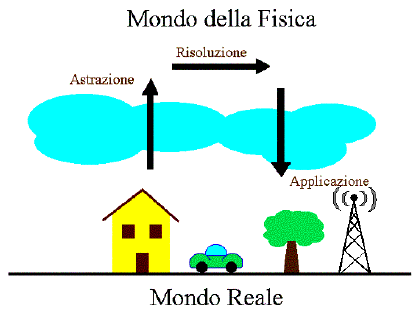
\includegraphics[scale = 0.5]{Relazione tra mondo fisico e mondo reale.PNG}
\end{figure} 


Dalla risoluzione all'applicazione, bisogna aggiungere le non idealità del mondo reale, che a sua volta, possono modificare anche l'astrazione matematica del mondo reale. \newline 

Le misure spesso si svolgono attraverso il confronto di grandezze omogenee (ad esempio nei tester si confronta la tensione da misurare con il riferimento di tensione all'interno di esso). \newline 

I riferimenti di misura sono costituiti dalle realizzazione delle definizioni di u.d.m. delle varie grandezze. \newline 

Prima di Maxwell, si prediligeva il riferimento usato dagli artefatti (ad esempio la il riferimento del chilogrammo di plato e lidio che si trova nel museo delle misure in Francia), 
mentre adesso si predilisce un riferimento assoluto, cioè basato su definizioni assolute, basate su fenomeni fisici o costanti di 
natura, che non dipendono dal tempo e dallo spazio, ritenuti "universali". \newline 

Se esiste la riferibilità, allora si può parlare di strumento di misura, sennò si parla di strumento di acquisizione. \newline 

Le relazioni tra grandezze e quindi tra u.d.m. sono esatte, poiché appartengono al mondo delle definizioni. \newline 

Le relazioni tra riferimenti di misura (realizzazioni pratiche delle u.d.m.), invece, 
non sono esatte perché i riferimenti sono affetti da imprecisioni e instabilità temporali. \newline 

L'imprecisione, vista come distanza tra realizzazione e definizione dell'u.d.m. (accuratezza) varia nel tempo. \newline 

Si impiega il termine errore nella teoria degli errori. \newline 

\newpage 

\section{Discussione qualitativa sull'incertezza di misura}
\footnote{Slide della prof | SDME 1.2 Metrologia - Introduzione | pag 16 - 25 \\  
Appunti | 2025-02-26 | pag 6 - 18}

Una grandezza fisica può essere determinata, e quindi conosciuta, soltanto ad un livello finito di incertezza. \newline 

Quanto più è bassa l'incertezza di misura, tanto più grande è il livello di conoscenza raggiunto. \newline 

Non esistono misure esatte perché l'incertezza di misura non potrà mai ridursi a zero. \newline 

Quindi si parla di incertezza di misura perché la misura comporta un intervallo di valori. \newline 

Si parla di errore solo durante la taratura di uno strumento di misura. \newline 

Quindi l'errore è diverso dall'accuratezza. \newline 

Possiamo esprimere le principali cause di incertezza: 

\begin{itemize}
    \item L'imprecisione intrinseca dei riferimenti rispetto ai quali si eseguono le misure 
    \item La conoscenza della relazione che esiste tra misurando e sistemi di misura è in genere incompleta 
    \item Le fluttuazioni naturali (rumore) limitano la risoluzione dei sistemi di rivelazione, cioè la capacità di distinguere stati vicini del misurando 
    \item La taratura per confronto o campioni di migliore qualità 
    \item Le misure avvengono in condizioni di non perfetta definizione, stabilità e controllo dei parametri ambientali, tra cui anche l'interazione dell'operatore 
    \item Gli strumenti possono presentare degli errori (ad esempio: errore di zero, errore di isteresi) 
\end{itemize}

Per essere uno strumento di misura, lo strumento deve essere riferibile rispetto alla grandezza primaria. \newline 

Quindi ci deve essere riferibilità e compatibilità. \newline 

Ci possono essere dei limiti tra strumento di misura e misurando. \newline 

Se ci sono dei valori empirici (e che quindi non si dimostrano), il valore di misura si porta dietro un'incertezza. \newline 

Il rumore comporta dei problemi nella misura perché il misurando varia nel tempo (si parla di processo stocastico). \newline 

Le fluttuazioni sono dei fenomeni generalmente distribuiti con una distribuzione gaussiana. \newline 

Inoltre, il rumore è ineliminabile. \newline 

Siccome il rumore è un processo stocastico, allora è necessario ripetere più volte la misura stessa. \newline 

In un qualunque sistema di misura, anche le u.d.m. fondamentali hanno una specifica realizzazione concreta (detta in francese mise en pratique) 
che presenta una incertezza quantificabile come lo scarto (accuratezza) rispetto alla definizione dell'u.d.m. stessa (riferimento ideale). \newline 

Tale scarto non si mantiene inalterato nel tempo (stabilità). \newline 

\newpage 

Le misure possono essere di due tipi: 

\begin{itemize}
    \item misure dirette, cioè il confronto di grandezze della stessa specie  
    \item misure indirette, cioè da un insieme di misure diverse si elabora il valore di una nuova grandezza
\end{itemize}

Non sempre è possibile una misura diretta e spesso si ricorre a una misura indiretta impiegando la relazione tra modello fisico e le varie grandezze: 
si pensi, ad esempio, alla misura della resistenza impiegando un voltmetro e un amperometro. \newline 

Avendoci a che fare con strumentazione digitale, uno dei problemi da affrontare è l'errore di quantizzazione. \newline 

Lo strumento digitale, in molti casi, è preferibile perché è più immune alle fluttuazioni dei rumori. \newline 

L'errore di quantizzazione è dovuto a strumentazione elettronica, acquisizione ed elaborazione dei segnali di tipo digitale, strumenti che includono l'ADC, e contatori elettronici. \newline 

In diversi casi è utile cambiare la risoluzione in base alla grandezza che si vuole misurare (c'è una differenza tra misurare $ \mu A$ in un circuito elettronico rispetto ai $M A$ di un impianto industriale). \newline 

La scelta della risoluzione ottimale alla misura è importante per capire se un segnale è informativo oppure se è rumore. \newline 

Utilizzando gli schemi a blocchi, possiamo rappresentare una misura come: 

\begin{figure}[h]
    \centering
    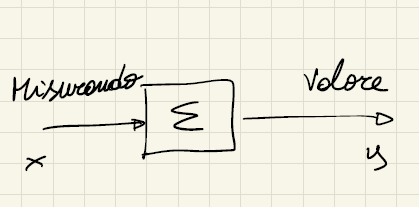
\includegraphics[scale = 0.5]{Schema a blocchi misura.PNG}
\end{figure} 

La relazione tra misurando e il valore della misura è di tipo lineare (almeno quelli che andiamo a considerare in questo corso), e quindi avremo una retta con una pendenza costante. \newline 

Possiamo scrivere: 

{
    \Large 
    \begin{equation}
        y = mx
    \end{equation}
    
}

La pendenza della retta misura la sensibilità dello strumento:

\begin{figure}[h]
    \centering
    \includegraphics[scale = 0.7]{Diverse sensibilità di uno strumento.PNG}
\end{figure} 

La maggiore sensibilità permette di misurare grandezze più piccole, più vicine al valore vero, 
allora l'uscita è facilmente leggibile. \newline 

Generalmente, un'elevata sensibilità deve essere accompagnata ad una elevata risoluzione. \newline 

In genere, in uno strumento di misura si richiede che l'uscita sia zero per segnali di ingresso nullo: 
l'errore di zero si ha quando questa condizione non è soddisfatta. \newline 

Inoltre, in uno strumento, può presentarsi un errore di isteresi, che è principalmente dovuto a sistemi di trasduzione che "immagazzinano" la carica precedente, dovuto ai componenti con memoria (come ad esempio un condensatore) presenti nello strumento stesso. \newline 

Dal punto di vista grafico, avremo un errore di isteresi in questo caso: 

\begin{figure}[h]
    \centering
    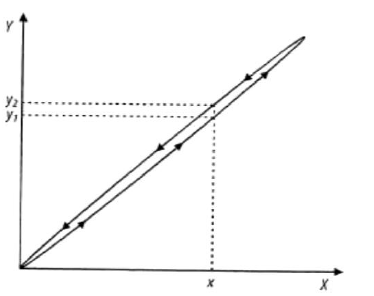
\includegraphics[scale = 0.5]{Errore di isteresi esempio.PNG}
\end{figure} 

\newpage 

\section{Un po' di terminologia} 
\footnote{Slide della prof | SDME 1.2 Metrologia - Introduzione | pag 26 - 29 \\  
Appunti | 2025-02-28 | pag 2}

Nella metrologia, il riferimento per la terminologia è il Dizionario di Metrologia, o Vocabolario Internazionale di Metrologia (VIM). \newline 

Per grandezza o quantità (misurabile) si intende un attribuito di un fenomeno o di una sostanza distinguibile qualitativamente e determinabile quantitativamente. \newline 

Dato un sistema di grandezze, si può costituire un sistema di grandezze se tra esse esistono relazione definite. \newline 

Per grandezze fondamentali (o di base) di un sistema si intende un insieme di grandezze convenzionalmente accettate come indipendenti. \newline 

Le grandezze derivate sono quelle grandezze che sono esprimibili attraverso le grandezze fondamentali. \newline 

Particolari grandezze possono adottate per convenzione come unità di misura. \newline 

Per misurando si intende una grandezza che si intende misurare. \newline 

Il risultato di una misura consiste nell'assegnare al misurando i seguenti valori: 

\begin{itemize}
    \item valore numerico 
    \item unità di misura 
    \item incertezza 
\end{itemize}

Per parametro si intende ogni caratteristica di un "sistema" alla quale è necessario assegnare valori 
per descrivere il sistema stesso, la sua evoluzione e/o le sue interazioni con altri sistemi e con l'ambiente. \newline 

Per segnale si intende la modificazione (o variazione) dello stato di un sistema usata per ottenere, elaborare e/o trasmettere un'informazione. \newline 

Per rumore, o disturbo, si intende la variazione della grandezza costituente il supporto di un segnale non correlata all'informazione da esso trasmessa. \newline 

Per incertezza si intende la stima quantitativa eseguita secondo procedimenti convenzionali, del nostro livello di non conoscenza del misurando. \newline 

Per accuratezza si intende il grado di concordanza tra un valore misurato e il valore "vero" di un misurando. \newline 

Generalmente, l'accuratezza viene data dal costruttore e/o dal laboratorio di taratura. \newline 

Si può definire l'accuratezza in base a cosa ci si riferisce: 

\begin{itemize}
    \item In riferimento ai campioni primari: è la stima dello scarto tra grandezza realizzata e definizione (esatta) dell'unità 
    \item In riferimento ad una misura: accordo che ci si attende tra il valore di misura e la migliore stima possibile per il misurando 
    \item In riferimento ad uno strumento specifico: valutazione delle differenze tra due misura di una stessa grandezza: la stima di un'incertezza dello strumento ottenuta mediante un'analisi precisa di tutte le cause di incertezza
\end{itemize}

Per ripetibilità o precisione si intende l'attitudine dello strumento o della misura a fornire, 
per uno stesso misurando, valori di lettura vicini tra loro, in letture consecutive eseguite in un breve intervallo di tempo, 
con lo stesso procedimento di misura, dallo stesso osservatore, nelle stesse condizioni per le grandezze di influenza e nello stesso luogo. \newline 

Per riproducibilità si intende la vicinanza di risultati ottenuti sullo stesso misurando in diverse specifici condizioni di misura, quindi possono cambiare principi e metodi di misura, osservatore, strumenti e riferimenti, luogo, tempo e condizioni.\newline

Per riferibilità si indica la proprietà di una misura di essere messa in relazione con quella fornita da un campione riconosciuto: si ottiene con una documentata catena ininterrotta di tarature. \newline 

Quindi, riferibilità è diversa da riproducibilità: la riferibilità è possibile, ad esempio, in un laboratorio dove si possono controllare tutti i parametri di misura, mentre la riproducibilità si ha quando si svolge la misura in campo, in un impianto di produzione. \newline 

Per sensibilità si intende il rapporto tra la variazione della grandezza (segnale) di uscita e la corrispondente variazione della grandezza (segnale) di ingresso. \newline 

Nel corso, andremo a studiare strumenti in cui la sensibilità è lineare e non dipende dal punto di lavoro (in quel caso si tratterebbe di strumenti non lineari). \newline 

Per risoluzione si intende la capacità dello strumento, o di una misura, di risolvere stati (livelli) diversi del misurando, senza alcuna particolare implicazione sulla capacità di valutare l'entità della variazione. \newline 

Per stabilità si intende l'attitudine di uno strumento o di una misura a fornire valori di lettura poco differenti tra loro in letture eseguite indipendente sullo stesso misurando in un intervallo di tempo definito e specificato. \newline 

In generale, prima di svolgere una misura, bisogna prima capire cosa si vuole misurare, studiare il fenomeno e, solo alla fine, si va a fare la misura con gli strumenti. \newline 

\newpage  

\section{Caratteristiche metrologiche di una misura o di uno strumento: definizioni} 
\footnote{Slide della prof | SDME 1.2 Metrologia - Introduzione | pag 30-32 \\  
Appunti | 2025-02-28 | pag 2 - 5}

Nel campo della misura, ci sono delle definizioni importanti (un po' da memorizzare come l'Ave Maria): 

\begin{itemize}
    \item Incertezza: stima quantitativa secondo procedimenti convenzionali, è il parametro che maggiormente caratterizza la qualità della misura stessa 
    \item Accuratezza: grado di accuratezza tra un valore misurato e il valore "vero" di un misurando 
    \item Ripetibilità o precisione: attitudine dello strumento o della misura a fornire per uno stesso misurando, valori di lettura vicini tra loro, in letture consecutive con lo stesso procedimento di misura 
    \item Riproducibilità: è la vicinanza di risultati ottenuti sullo stesso misurando in diverse condizioni di misura 
    \item Riferibilità: indica la proprietà di una misura di essere messa in relazione con quella fornita da un campione riconosciuto 
    \item Sensibilità: rapporto tra la variazione della grandezza (segnale) di uscita e la corrispondente varazione della grandezza (segnale) di ingresso 
    \item Risoluzione: capacità dello strumento, o di una misura, di risolvere strati (livelli) diversi del misurando 
    \item Stabilità: attitudine di uno strumento o di una misura a fornire valori di lettura poco differenti tra loro in letture eseguite indipendentemente sullo stesso misurando in un intervallo di tempo definito e specificato
\end{itemize}

\newpage